\chapter{Implementierung}
In diesem Kapitel wird zunächst die Implementierung der verschieden Ansätze in C++ behandelt. Hierbei wird auch auf die Besonderheiten des FPGA eingegangen. Des weiteren wird erläutert, wie der FPGA programmiert wird, vor allem in Hinblick auf die Parallelisierung der einzelnen Komponenten. Eine einzelne Instanz der logistischen Regression wird im Folgenden als Perceptron bezeichnet.
\section{Implementierung in C++}
Für die erste Implementierung der Voraussagefunktion wurde der Code von \cite{IMPL} aus Python in C++ übersetzt und an die Eigenschaften eines FPGA angepasst. In Abbildung 4.1 sind die Kernfunktionen des Programmcodes dargestellt. Die Funktion \textit{predict()} liefert die Berechnung der Formel $\dfrac{1}{1+\exp(-(\beta_0+x_i^T\beta))}$. Die Koeffizienten $\beta$ sind hier als Array $coefficients[\text{ }]$ gespeichert, zudem gibt es für die Batch-Realisierung ein Hilfsarray $tmp\textit{\_}coefficients[\text{ }]$. Der Datentyp \textit{DATA\_TYPE} kann hier zum einen Als Gleitkommazahl (\textit{float}), zu anderen als Fixkommazahl (\textit{ap\_fixed}) deklariert werden. Die Wahl für den Fixkomma-Datentyp fällt auf ein von Xilinx selbst bereitgestelltes Konstrukt \textit{ap\_fixed}, da es für das FPGA optimiert wurde und hier eine Vielzahl an Konfigurationen vorgenommen werden können. Die Gesamtanzahl der für eine Instanz belegten Bits wurde auf 16 festgelegt, davon ein Vorzeichenbit und 4 Vorkommastellen. Durch die Einstellung \textit{AP\_RND\_CONV} wird die Zahl, zum Beispiel nach einer Divisionsberechnung auf den nächsten repräsentierbaren Wert gerundet. Die Rundungsrichtung ist dabei abhängig von dem am wenigsten signifikanten Bit. Ist dieses gesetzt wird gegen $+\infty$, andernfalls gegen $-\infty$ gerundet \cite{XIL2}.
Um einem eventuellen Overflow der Zahl entgegenzuwirken wählt man die Einstellung \textit{AP\_SAT\_SYM}. Im Fall eines Positiven Overflows wird hierbei der höchste, bei einem negativen Overflow der kleinste darstellbare Wert gewählt.\cite{XIL2} Die FPGA Einstellung \textit{pragma HLS LOOP FLATTEN} sorgt für eine Parallelisierung der Schleife auf dem FPGA. Das funktioniert allerdings nur, wenn innerhalb der Schleife auf immer andere Ziele geschrieben wird.\\ In der Funktion \textit{predict()} zum Beispiel wird die Variable \textit{yhat} immer wieder neu gesetzt, sodass eine Paralleliserung hier nicht möglich ist. 
\begin{figure}[ht]
\centering
\begin{lstlisting}
/* Voraussage treffen anhand logistischer Regression */
DATA_TYPE predict(){
    DATA_TYPE yhat = coefficients[0];
	for(int i=0; i<FEATURE_COUNT; i++){
		yhat+=coefficients[i+1]*features[i];
	}
	float tmp_yhat=-yhat;
	DATA_TYPE predicted=1.0f/(1.0f+hls::expf(tmp_yhat));
	return predicted;
}
\end{lstlisting}
\begin{lstlisting}
void learn(){
    DATA_TYPE predicted=predict();
    DATA_TYPE error=label-predicted;
    tmp_coefficients[0]+=error;
	for(int i=0; i<FEATURE_COUNT; i++){
		#pragma HLS LOOP FLATTEN
		tmp_coefficients[i+1]+=error*features[i];
	}
	/* Batch Update der Koeffizienten */
	batch_count++;
	if(batch_count>=BATCH_SIZE){
		batch_count=0;
		coefficients[0]+=lrate*tmp_coefficients[0]/BATCH_SIZE;
		tmp_coefficients[0]=0;
		for(int i=1; i<FEATURE_COUNT+1; i++){
			#pragma HLS LOOP FLATTEN
			coefficients[i]=punish(i) + 
				lrate*tmp_coefficients[i]/BATCH_SIZE;
			tmp_coefficients[0]=0;
		}
	}
}
\end{lstlisting}
\caption{Codes des Perzeptrons}
\end{figure}
\\Die Funktion \textit{hls::expf()} wird von Xilinx geliefert und dient als Realisierung der Expotentialfunktion und ist für FPGAs optimiert.\\ 


Um die High-Performance Schnittstelle über PCIe von \cite{DILL} voll ausnutzen zu können wurde eine Trennung der Codeteile vorgenommen, damit ein Teil des Algorithmus auf dem FPGA und ein Teil auf dem Hostcomputer laufen kann. Der Hostrechner übernimmt hier die Vorbereitung der Daten und die äußeren Schleifendurchläufe. Es werden immer die einzelnen Variablen mit dem dazugehörigen Label an den FPGA gesendet, welcher dann je nach Konfiguration damit trainiert oder eine Voraussage trifft. Der Vorteil hierbei ist, dass auf dem FPGA mehrere logistische Regressionen gleichzeitig implementiert sind, die mit verschiedenen Parametern (zum Beispiel einem C für die Fehlerbestrafungsgewichtung oder unterschiedlichen Lernraten) initialisiert wurden.\\
Die Methode \textit{punish()} wendet die ausgewählte Regularisierungsmethode auf das Batch Update an. Es wurden keine Regularisierung, L1- und L2-Regularisierung implementiert, sodass für den selben Trainingsdurchlauf verschiedene Methoden getestet werden können. in Abbildung 4.2 ist die Funktion als Programmcode dargestellt.\\
\begin{figure}[ht]
\centering
\begin{lstlisting}
/*Punishment sollte vorinitialisiert werden, da Konstant abhaengig von der Regularisierungsgewichtung, der Batchgroesse und der Lernrate */

DATA_TYPE punishment=lrate*c/BATCH_SIZE

void punish(int i){
	/*L1 Regularisierung*/
	if(method==1){
		return coefficients[i]-punishment*sign(coefficients[i]);
	}
	/*L2 Regularisierung*/
	if(method==2){
		return coefficients[i]*(1-punishment);
	}
	return coefficients[i];
	    
}
\end{lstlisting}
\caption{Implementierte Regularisierungsmethoden}
\end{figure}\\
Die angewendete L1- und L2-Regularisierung für das Koeffizientenupdate ergibt sich aus der Ableitung der Kostenfunktion, welche um den Regularisierungsterm erweitert wurde.
für LASSO ergibt sich der Term aus:
\begin{displaymath}
\beta_i^{(l+1)}=\beta_i^{(l)}+\eta^{(l)} \cdot \dfrac{\partial}{\partial \beta_i} \left( J(\beta)-\frac{C}{m} \cdot | \beta_i^{(l)} |\right)
\end{displaymath}
Mit $x_i \in \vec x_l$. Da die Betragsfunktion nicht differenzierbar ist behilft man sich mit der Vorzeichenfunktion \textit{sign()}. Es entsteht damit folgender Term für das Update \cite{L1C}:
\begin{displaymath}
\beta_i^{(l+1)} = \beta_i^{(l)} + \eta^{(l)} \cdot \frac{1}{m} \sum_{i=l\cdot m + 1}^{(l+1) \cdot m} (y_i-\pi(\vec x_i)) \cdot x_i -\eta^{(l)}\cdot \frac{C}{m} \cdot sign(\beta_i^{(l)})
\end{displaymath}
Für die Ridge Regression ist der Ableitungsterm deutlich einfacher zu bestimmen. Aus 
\begin{displaymath}
\beta_i^{(l+1)}=\beta_i^{(l)}+\eta^{(l)} \cdot \dfrac{\partial}{\partial \beta_i} \left( J(\beta)-\frac{C}{2m} \cdot \sum_{k=1}^d (\beta_k^{(l)})^2 \right)
\end{displaymath} wird \cite{HER2}
\begin{displaymath}
\beta_i^{(l+1)} = \beta_i^{(l)} \cdot \left(1-\eta^{(l)}\frac{C}{m}\right) + \eta^{(l)} \cdot \frac{1}{m} \sum_{i=l\cdot m + 1}^{(l+1) \cdot m} (y_i-\pi(\vec x_i)) \cdot x_i
\end{displaymath}\\
Um die Datenverteilung auf dem FPGA zu gewährleisten wurde sowohl eine Verteiler- als auch eine Sammlerklasse implementiert. Diese sind für dafür zuständig den Datenstrom von Daten und Konfigurationsparametern auf die jeweiligen Perceptrons zu verteilen beziehungsweise von diesen einzusammeln. Die Sammlerklasse markiert zusätzlich noch die ausgegebenen Daten mit der Identifikation des jeweiligen Perceptrons, damit die Ergebnisse nach einem Durchlauf zugeordnet werden können.
Die Verteilerklasse übernimmt bei der Implementierung mit der 16-Bit Fixkommazahl zudem die Aufteilung des Eingangstroms, da über die 32-Bit Ausgangsleitung des Xillybus-Blocks jeweils zwei Datenpunkte pro Übertragung versendet werden können.
\section{Implementierung als Blockdesign}
Um Auf dem FPGA zu implementieren, muss der Code für den Verteiler, den Sammler und das Perceptron in eine IP (Intelectual Property) umgewandelt werden. Die IP-Blöcke werden für das Blockdesign wie in Abbildung 4.5 angeordnet und verbunden. Hierbei sind die Perceptrons für Daten aus der MNIST (Modified National Institute of Standards and Technology) Datenbank konfiguriert, das heißt jedes Perceptron hat einen Variablenspeicher von 784 Features (28x28 Pixel) und jeweils 785 Koeffizienten und Hilfskoeffizienten.\\
Die MNIST Datenbank ist eine Sammlung handgeschriebener Ziffern, komprimiert, zentriert und normalisiert auf 28x28 Pixel mit Werten zwischen 0-256, welche die Farben von Weiß nach Schwarz repräsentieren. Die 60.000 Trainingsvariablen wurden zu jeweils gleichen Teilen aus der NIST (National Institute of Standards and Technology) Testdatenbank und der NIST Trainingsdatenbank entnommen, gleiches gilt für die 10.000 Variablen große Testmenge. Diese Anpassung wurde vorgenommen, da die Variablen der Testmenge unter Mitarbeitern des Volkszählungsamts erhoben wurden und deutlich besser zu klassifizieren sind als die unter Studenten erhobenen Daten der Trainingsmenge. Die Daten der Trainingsmenge wurden von circa 250 Teilnehmern erhoben, von denen keine Einträge in der Testmenge eingefügt wurden \cite{MNIST}.\\
\begin{figure}[ht]
\centering
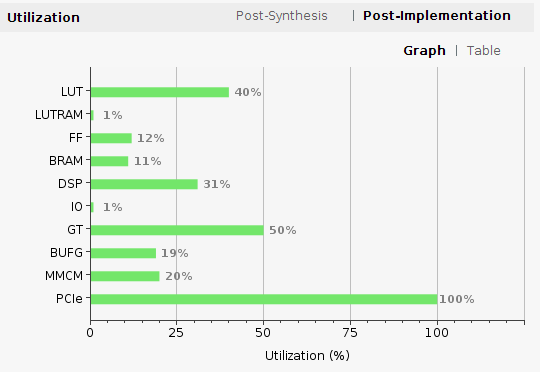
\includegraphics[scale=0.9]{bilder/auslastung1}
\caption{Auslastung auf dem FPGA mit 16-Bit Fixkommazahl und 8 Perceptrons}
\end{figure}\\
Die Auslastung des FPGA für diese Implementierung beträgt in etwa 50\% (siehe Abbildung 4.3), sodass auch 16 Perceptrons parallel geschaltet werden können. Für die bildliche Darstellung in dieser Arbeit wäre dies jedoch ein zu großes Diagramm. 
Die Auslastung für 16 Perceptrons unter MNIST beträgt 90\% der LUT und ist in Abbildung 4.4 veranschaulicht. \\
\begin{figure}[ht]
\centering
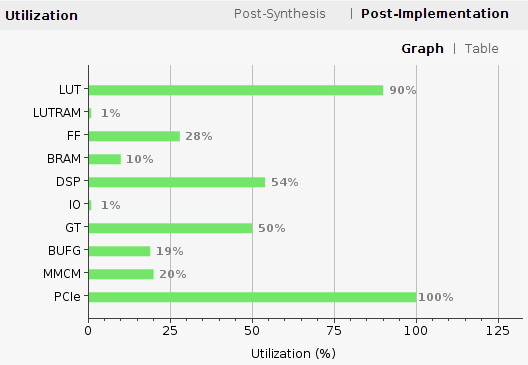
\includegraphics[scale=0.95]{bilder/auslastung2}
\caption{Auslastung auf dem FPGA mit 16-Bit Fixkommazahl und 16 Perceptrons}
\end{figure}\\ 
\begin{figure}
\centering
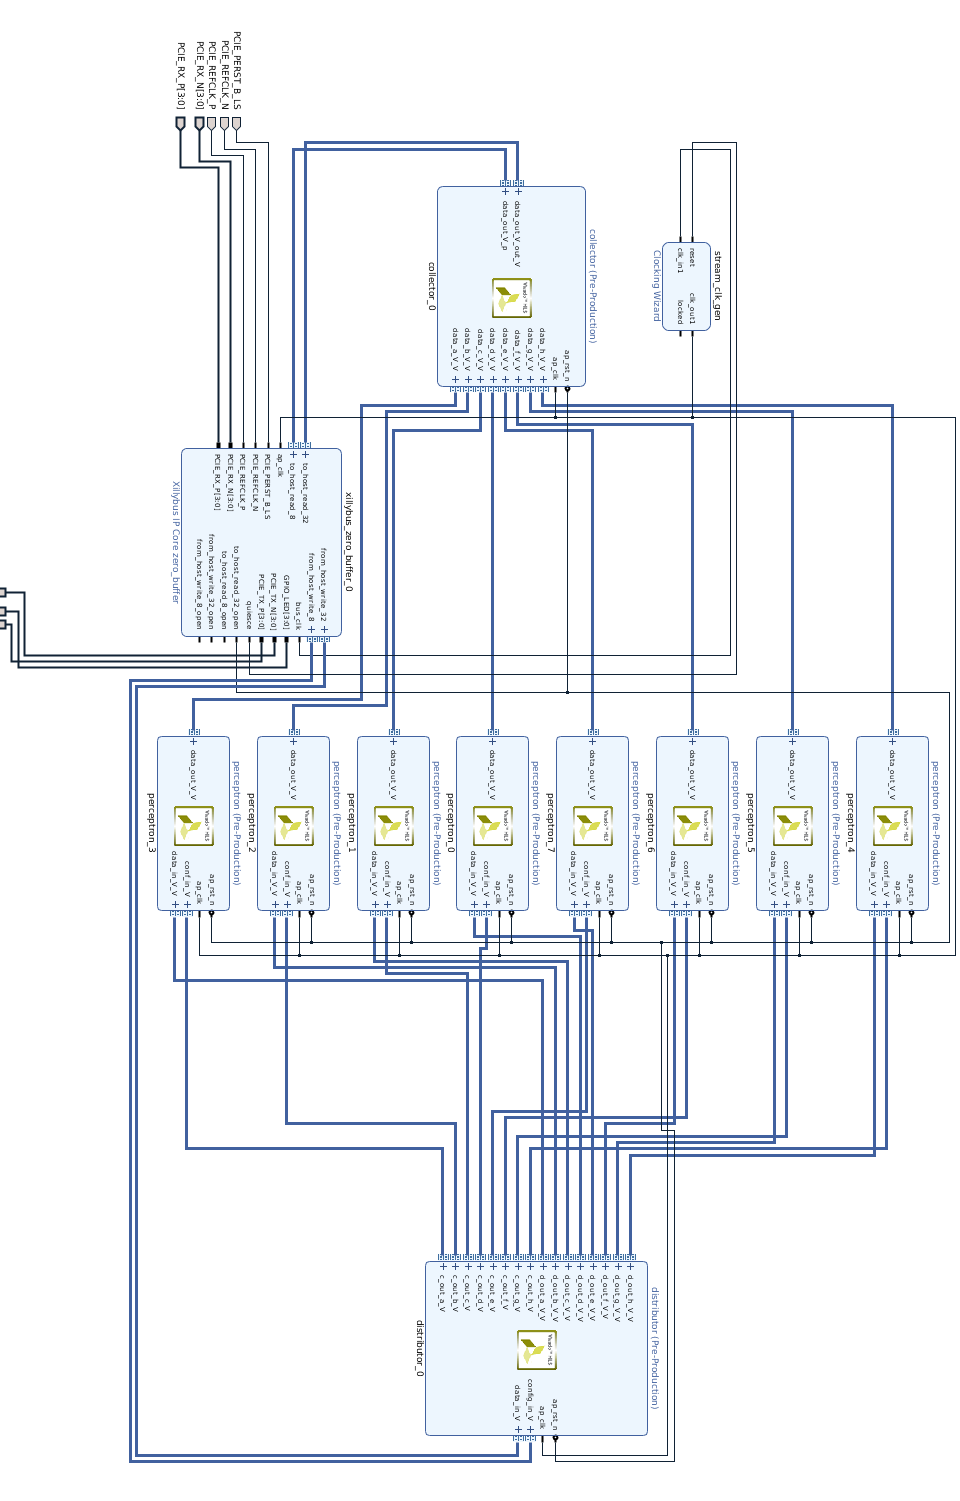
\includegraphics[scale=0.7]{bilder/blockdesign}
\caption{Das Blockdesign auf dem FPGA}
\end{figure}\newpage
Für Datensätze mit mehr Features als MNIST erhöht sich zudem die Auslastung, da jedes Perceptron zwei Koeffizientenvektoren und einen Zwischenpuffer mit einer Länge gleich der Anzahl der Features im Speicher haben muss. Daher können für diese Datensätze keine 16 oder sogar weniger als 8 Perceptrons in das Design eingefügt werden.
Bei mehr als 16 Perceptrons treten zudem einige Probleme bezüglich des Timings auf, welche in Kapitel 5 näher behandelt werden.

\section{Implementierung der Hostanwendung}
Durch die Nutzung der PCIe-Schnittstelle mit Xillybus wie in \cite{DILL} ausgeführt muss die Hostanwendung einiges mehr leisten als nur den Datenaustausch zwischen Hostrechner und FPGA zu verwalten. Sie dient der Aufbereitung der Daten, der Koordination mit dem FPGA und der Auswertung der Ergebnisse. Es werden zunächst die Eingabedaten in den Speicher geladen und auf Werte zwischen 0 und 1 normalisiert. Dann werden die Werte in das angegebene Zahlenformat konvertiert. Je nach Datensatz ist dies ein nicht unerheblicher Zeitaufwand, der jedoch unvermeidlich ist.\\
Um den FPGA nun auf das Lernen eines neuen Modells vorzubereiten können jetzt die Umgebungsvariablen gesetzt werden. Jedes Perceptron ist separat konfigurierbar, womit dem Nutzer eine Vielzahl von Testmöglichkeiten eröffnet werden. Regulierbar sind der Hyperparameter $C$, die Lernrate des Modells, die Batchgröße für den Gradientenabstieg und die Regularisierungsmethode. Alle diese Werte werden in das gewählte Zahlenformat konvertiert, sodass zum Beispiel eine Batchgröße von 5 im Zahlenformat $ap\_fixed<16,3>$ (16 Bit Fixkommazahl mit 3 Vorkommabits, davon ein Vorzeichenbit) nicht angegeben werden kann. für diesen Fall kann die Batchgröße auf 0 gesetzt und das Batchupdate nach der gewünschten Trainingsmenge manuell vom Hostrechner aus initiiert werden. Die hohe Konfigurierbarkeit hat den Vorteil, dass viele verschiedene Einstellungen auf dem FPGA getestet werden können, ohne dass dieser neu programmiert werden muss. Das Erstellen von Pareto-Fronten ist also gut umzusetzen.\\
Auch die Koeffizienten müssen durch das Hostprogramm vorbelegt werden. Das kann durch einen Nullvektor oder durch Normalverteilte Zufallszahlen geschehen, bietet aber auch die Möglichkeit bereits trainierte Koeffizienten zu verwenden. Durch das Einstellen der Laufvariable auf 0 kann hiermit ein Trainingsvorgang übersprungen werden.\\
Die Implementierung mit dem Fokus PCIe Schnittstelle erfordert es, dass für jede Operation auf dem FPGA zunächst alle Features einer Variable übertragen werden müssen. Jedes Perceptron auf dem FPGA besitzt einen Pufferspeicher für genau eine Variable, sodass mit dem Übertragen eines Datenpunktes alle 8(16) Perceptrons initialisiert werden können. Dieser Puffer wird sowohl für die Trainings- als auch für die Testdaten verwendet, um möglichst wenig von dem stark begrenzten Speicherplatz des FPGA zu verwenden.
Aufgrund technisch bedingter Schwierigkeiten (in Kapitel 5 werden diese behandelt) Werden die Trainings- und die Testmethode in verschiedenen Prozeduren behandelt. 
\subsection{Training}
Das Trainingsprogramm hat die Aufgabe das FPGA auf den Start eines neuen Trainingszyklus' vorzubereiten und diesen dann durchzuführen. Die wichtigsten Programmteile werden in folgendem Codeteil vorgestellt:
\begin{figure}[ht]
\centering
\begin{lstlisting}
/*Konfiguriere den FPGA mit Daten aus der Config-Datei*/
write(fc, conf, sizeof(char));
write(fc, NULL,0);
	for(int i =0; i< PERCEPTRONS; i++){
		write(fdw, &hyper[i], sizeof(DATA_TYPE));
		write(fdw, &lrate[i], sizeof(DATA_TYPE));
		write(fdw, &batch[i], sizeof(DATA_TYPE));
		write(fdw, &modus[i], sizeof(DATA_TYPE));
		write(fdw, NULL,0);
	}
/*Normalverteilte Zufallszahlen zur Koeffizienteninitialisierung*/
	for(int i=0; i<((FEATURE_COUNT+1)); i++){
		DATA_TYPE t =nd_random.dev();
		rc = write(fdw, &t, sizeof(DATA_TYPE));
		write(fdw, NULL,0);
	}
\end{lstlisting}
\caption{Konfiguration des FPGA}
\end{figure}\\
Die Filestreams \textit{fc} und \textit{fdw} sind die Outputstreams in die Devicefiles der Xillybus-Schnittstelle. Eine Schreiboperation mit \textit{NULL} und einer Länge von 0 (\textit{write(fc, NULL, 0)}) sorgt hier für das leeren der Internen Puffer, sodass die geschriebenen Daten dem FPGA zur Verfügung stehen. Die Koeffizienten werden durch \textit{nd\_random.dev()} normalverteilte Pseudozufallszahlen initialisiert, da man davon ausgeht dass die gelernten Koeffizienten später auch normalverteilt sind.\\
Der Trainingsvorgang selbst besteht aus einer Doppelschleife über die Epochen und die einzelnen Zyklen. In jeder Epoche werden alle Zyklen exakt gleich durchgeführt. Dies ist über die Deaktivierung der Methode \textit{srand(seed)} abzuschalten, sodass in jeder Epoche ein völlig anderer Trainingszyklus (mit neuen und anders sortierten Daten) ablaufen kann.\\
\begin{figure}
\centering
\begin{lstlisting}
/*Starte Epochen*/
for(int lauf =0; lauf<max_runs;lauf++){
/*Zufallsgenerator neu seeden*/
	srand(seed);
/*Starte Trainingszyklus*/
	for(int cycle=0; cycle < max_runs; cycle++){
/*Zufaellige Position in der Trainingsmenge bestimmen*/
		int idx = rand() % number_of_labels_train;
		int idx_data= idx*FEATURE_COUNT;
		rc = write(fc, conf+2, sizeof(char));
		write(fc, NULL, 0);

/*Alle Features und das Label versenden*/
		for(int i=0;i<FEATURE_COUNT;i++){
			DATA_TYPE st = train_set[idx_data+i];
			rc = write(fdw, &st, sizeof(DATA_TYPE));
			write(fdw, NULL,0);
		}
		DATA_TYPE st = train_label[idx];
		rc = write(fdw, &st, sizeof(DATA_TYPE));
		write(fdw, NULL,0);
	    if (rc <= 0) {
	    	perror("write() failed labels");
	        exit(1);
	    }
	}
/*Batch Updaten wenn keine Groesse angegeben ist*/
	if(batch_is_zero){
		for(int i=0; i< PERCEPTRONS; i++){
			if(batch[i] == zero){
				rc = write(fc, conf+1, sizeof(char));
				rc = write(fc, perceptron_names+i, sizeof(char));
				write(fc, NULL, 0);
			}
		}
	}
}
\end{lstlisting}
\caption{Durchführen der Trainingszyklen}
\end{figure}\newpage

\subsection{Vorhersagen}
Sobald das Modell auf dem FPGA trainiert ist kann mit den Voraussagetests begonnen werden. Es werden dafür alle Variablenpuffer der Perceptrons mit der zu testenden Variable gefüllt. Nun muss für jedes Perceptron der Aufruf zum Vorhersagen erfolgen. Die Lese- und Schreiboperationen können in verschiedenen Threads ausgeführt werden um Zeit zu sparen. Dabei ist es nötig zu wissen in welcher Reihenfolge die Perceptrons ihre Ausgaben an den Hostrechner senden. Durch das einzelne Anstoßen der Vorhersagefunktion ist dies gewährleistet. Zudem ist \textit{read()} eine blockierende Funktion, sodass keine Daten übergangen werden.\\
Die ausgelesenen Ergebnisse werden in einer Datei abgelegt, ohne diese vorher zu leeren. \\
\begin{figure}[ht]
\centering
\begin{lstlisting}
/*Gemeinsamen Speicher reservieren*/
DATA_TYPE *right = (DATA_TYPE *)mmap(NULL, maxruns*sizeof(DATA_TYPE), protection, visibility, -1, 0);
  DATA_TYPE *d_pred = (DATA_TYPE *)mmap(NULL, PERCEPTRONS*maxruns*sizeof(DATA_TYPE),protection, visibility, -1, 0);
/*Elternprozess starten*/
  pid_t pid = fork();
  if(pid){
    for(int i =0; i<maxruns; i++){
      int idx_p=i+offset;
      if(offset<0){
        idx_p= rand() % (number_of_labels_test);
      }
      right[i] = test_label[idx_p];
      write(fc, &load, sizeof(char));
      write(fc, NULL, 0);
      for(int j=0; j<MAX_FEATURE_COUNT;j=j+1){
        int idx = (idx_p*MAX_FEATURE_COUNT+j);
        DATA_TYPE st = test_set[idx];
        write(fdw, &st, sizeof(DATA_TYPE));
        write(fdw, NULL, 0);
      }
      for(int j=0;j<PERCEPTRONS; j++){
        write(fc, &test , sizeof(char));
        write(fc, ar+j, sizeof(char));
        write(fc, NULL, 0);
      }
    }
    wait(NULL);
  }
\end{lstlisting}
\caption{Elternprozess der Trainingsmethode}
\end{figure}\\
\begin{figure}[ht]
\centering
\begin{lstlisting}
...
  if(pid){
  	...
  } 
  else{
    for(int i =0;i<maxruns;i++){
      for(int j=0;j<PERCEPTRONS;j++){
        read(fdr_c, conf, sizeof(char));
        read(fdr_d, d_pred+(j*maxruns+i) ,sizeof(DATA_TYPE));
      }
    }
    _exit(0);
  }
\end{lstlisting}
\caption{Kindprozess der Trainingsmethode}
\end{figure}\\
Zu den extrahierten Ergebnissen gehören die Trefferquoten der Vorhersagen über die eingegebenen Daten, die richtigerweise richtig klassifizierten ("`true positive"'), die fälschlicherweise als richtig bezeichneten  ("`false positiv"'), die richtigerweise als falsch klassifizierten  ("`true negative"') und die fälschlicherweise als falsch deklarierten ("`false negativ"') Daten.\\
\subsection{Koeffizienten}
Wenn ein Modell soweit trainiert worden ist dass es zufriedenstellende Vorhersagen treffen kann, dann speichert man die Koeffizienten für die weitere Verwendung oder zur Analyse ab. Auf normalen Rechnern kann man sie in Dateien überspielen lassen oder in die Ausgabe leiten. Von einem FPGA
müssen die Koeffizienten jedoch erst extrahiert werden um weiter mit ihnen arbeiten zu können. Die Implementierung bietet dazu eine Methode an, die jederzeit den Koeffizientenvektor des gewünschten Perceptrons ausgeben kann. Auch nach dem Schließen der Systemdateien von Xillybus, und damit dem löschen der Puffer bleibt der letzte Zustand des FPGA auf diesem erhalten. Sogar nach einem Neustart des Hostrechners sind die Koeffizienten noch im jeweiligen Perceptron hinterlegt. Demnach kann das Modell beliebig weiter bearbeitet oder zum testen und vorhersagen von Daten benutzt werden, bis es sich durch seine Performance für eine Extraktion qualifiziert.\\
Der Code des Extraktors ist hier aufgeführt: 

\begin{figure}[ht]
\centering
\begin{lstlisting}
char *ct_coef = (char*)malloc(sizeof(char)*PERCEPTRONS*(FEATURE_COUNT+1));
DATA_TYPE *dt_coef = (DATA_TYPE*)malloc(sizeof(DATA_TYPE)*(FEATURE_COUNT+1)*PERCEPTRONS);

int s_coef = (FEATURE_COUNT+1);
for(int j=0; j<PERCEPTRONS;j++){
  write(fc, &conf, sizeof(char));
  write(fc, perceptron_names+j, sizeof(char));
  write(fc, NULL, 0);
  for(int i=0;i<s_coef;i++){
    read(fdr_c, &config, sizeof(char));
    ct_coef[j*s_coef+i]=config;
    read(fdr_d, &fbuf ,sizeof(DATA_TYPE));
    dt_coef[j*s_coef+i] = fbuf;
  }
}
printf("open datafile");
ofstream dw ("coeff.txt", std::ofstream::trunc);
if (dw.is_open()){
  for(int j=0;j<PERCEPTRONS;j++){
    bool first = true;
    int count_c=0;
    for(int i=0;i<(MAX_FEATURE_COUNT+1)*PERCEPTRONS;i++){
      if(ct_coef[i] == perceptron_names[j]){
        if(first){
          dw << dt_coef[i] << "\n";
          first=false;
        }
        else{
          count_c++;
          if(count_c % 28 == 0 )
            dw << dt_coef[i] << "\n";
          else
            dw << dt_coef[i] << ",";
        }
      }
    }
  }
  dw.close();
}
\end{lstlisting}
\caption{Extraktion der Koeffizienten}
\end{figure}